\documentclass{msuposter}
\usepackage{lipsum}
\usepackage{tikz,wrapfig}

%% REQUIRED
\title{Sample Poster Made with {\ttfamily msuposter.cls}}
\author{Your Name Here}
\institute{AMS Graduate Student Chapter}

%% OPTIONAL
\advisor{Name, Department of Mathematics}

%% SET COLUMN WIDTH
\newcommand{\colwidth}{0.3\linewidth}

\begin{document}
\begin{frame}{}
\begin{columns}[t]

\begin{column}{\colwidth}

\begin{block}{Introduction}
Type your introduction to your research here.
\end{block}

\begin{block}{Section 1}
Use the {\ttfamily block} environment to create different sections for your poster. 
\end{block}

\begin{block}{Section 2} 
You can fill in the existing blocks by typing in the spaces between {\ttfamily\textbackslash begin\{block\}} and {\ttfamily\textbackslash end\{block\}}.\cite{NIPS2014_5ca3e9b1}
\end{block}

\begin{block}{\bfseries Section 3}
Change the title of the block by editing the brackets immediately following {\ttfamily\textbackslash begin\{block\}\{...\}}.  By default, the block title will not be bold.  If you'd like to make it bold you may add {\ttfamily \textbackslash bfseries} at the front of the title.
\end{block}

\begin{block}{Citations}
It's important to use cite any references you have.  Here is an example citation \cite{cite1}.
\end{block}

\begin{block}{Lists}
Numbered lists may be created as such:
\begin{enumerate}
  \item This is item one.
  \item This is item two.
  \item This is item three.
\end{enumerate}

Unnumbered lists may be created as such:
\begin{itemize}
  \item Here's an item!
  \item Here's an item!
  \begin{itemize}
    \item Here's a sub-item!
  \end{itemize}
  \item Here's an item!
\end{itemize}
\end{block}

\begin{block}{Tables}

Here is an example of a table:
\begin{table}\centering
\caption[Table short caption]{The first table}
\begin{tabular}{r|l c}
  Col 1   & Col 2  & Col 3 \\\hline
  This    & This   & This \\
  Column  & Column & Column \\
  Is      & Is     & Is \\
  Right   & Left   & Centered \\
  Aligned & Aligned
\end{tabular}
\end{table}

\end{block}

\end{column}

%% COLUMN DIVIDE %%%%%%%%%%%%%%%%%%%%%%%%%%%%

\begin{column}{\colwidth}

\begin{block}{Figures}
You can use the {\ttfamily tikz} package to draw figures.  Here's an example:
\begin{figure}\centering
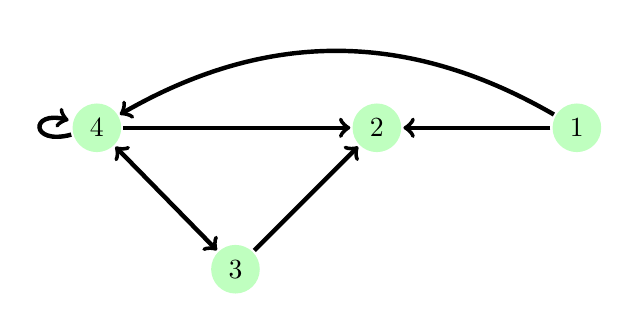
\begin{tikzpicture}[ultra thick,my node/.style={circle,fill=green!25},node distance=1in]
  % NODES
  \node[my node] (node1) {1};
  \node[my node] (node2) [left of=node1] {2};
  \node[my node] (node3) [below left of=node2] {3};
  \node[my node] (node4) [left of=node2,node distance=1.4in] {4};
  % PATHS
  \path[->] 
   (node1) edge (node2)
           edge[bend right] (node4);
  \path[<-] 
   (node2) edge (node3)
           edge (node4);
  \path[<->] 
   (node3) edge (node4);
  \path 
   (node4) edge[loop left] (node4);
\end{tikzpicture}
\caption[Figure short caption]{Look at that awesome directed graph!}\label{fig:coolgraph}
\end{figure}

You can also include outside graphics:
\begin{figure}\centering
  
\includegraphics[scale=1]{spartans.jpg} %change scale to change size, or use [width=##, height=##]
  \caption{Check out that Spartan S!}\label{fig:flyingC}
\end{figure}

In order to refer back to the figures, you can label them with {\ttfamily\textbackslash label\{...\}}, and then refer to them with {\ttfamily\textbackslash ref\{...\}}.  For example, I really like Figure \ref{fig:coolgraph} and Figure \ref{fig:flyingC}.

And if you want to wrap text around figures, you can use the {\ttfamily wrapfig} package.  For example:

\begin{wrapfigure}{r}{0.5\textwidth}
  \centering
    
\includegraphics[width=0.25\textwidth]{spartans.jpg}
  \caption{A 2nd Spartan S!}
\end{wrapfigure}

\lipsum[1-2] % this command just inserts nonsense text so you can see the text wrapping

\end{block}

\begin{block}{Mathematics}
Mathematics may be formatted as usual.  We may wish to include some math within the text of our document.  This can be accomplished as such: $x^{3} + 2x - 4$ is a polynomial.  On the other hand, we may sometimes wish to have the mathematics displayed more prominently:
\[
  f(x) = x^{3} + 2x - 4.
\]
A good example that highlights how to handle fractions and square roots is the Quadratic Formula:
\[
  x = \frac{-b \pm \sqrt{b^{2} - 4ac}}{2a} \quad\text{where } a,b,c \in \mathbb{R}.
\]
That example also illustrates that {\ttfamily \textbackslash text\{...\}} in math mode is consistent with the normal text.  Let's make sure big operators look good:
\[
  \int_{a}^{b} f(x) dx = \lim_{\max \Delta x_{k} \to 0} \sum_{k=1}^{n} f(x_{k}^{*}) \Delta x_{k}
\]
\end{block}

\end{column}

%% COLUMN DIVIDE %%%%%%%%%%%%%%%%%%%%%%%%%%%%

\begin{column}{\colwidth}

\begin{block}{Other Types of Blocks}
In addition to the standard {\ttfamily block} environment, there are a handful of other block styles you may use.  Some examples are:
\begin{itemize}
 \item Environments from the {\ttfamily amsthm} package (e.g., {\ttfamily theorem}, {\ttfamily definition})
 \item {\ttfamily exampleblock}
 \item {\ttfamily alertblock}
\end{itemize}
\end{block}

\begin{definition}[My Definition]
Here is a definition that is necessary to understand my research...
\end{definition}

\begin{theorem}[My Theorem Title]
Here's a theorem that I proved...  Note that this text is automatically italicized.
\end{theorem}

\begin{exampleblock}{An Example Block}
Here is an example that is highly insightful...  Note that this style of block will automatically change the block's colors.
\end{exampleblock}

\begin{alertblock}{An Alerted Block}
Here is something that is extremely important!  Note that this style of block will automatically change the block's colors.
\end{alertblock}

%% ACKNOWLEDGEMENTS
\begin{block}{Acknowledgements}
Make sure to include an acknowledgement section that recognized those that have helped in your work. Include any grant numbers here. 
\end{block}

%% REFERENCES (except size if need be)
\begin{block}{References} %%% INSERT YOUR REFERENCES IN THE BIB FILE
\scriptsize
\bibliography{references}
\bibliographystyle{plain}
% \end{scriptsize}
\end{block}

%%%% end of references %%%%%%%%%%%%%%%%
\end{column}

\end{columns}
\end{frame}
\end{document}
